\chapter{进程和线程管理}\label{ch:process-and-thread-management}

\section{进程和线程概述}\label{sec:4-process-and-thread-overview}

进程（Process）和线程（Thread）是 RME 对其上执行的程序提供的基本抽象。RME 的进程和线程抽象层次较低，这与 Linux 等传统操作系统的高层次抽象实现是非常不同的。与传统操作系统相比，RME 的实现具备更高的灵活性和性能。

\subsection{进程概述}\label{subsec:4-process-overview}

在 RME 中，一个进程指的是拥有一个独立地址空间\footnote{也即一个独立页表}和一个权能表的最小保护域（Protection
Domain）。页表决定了进程的地址空间，权能表则决定了该进程中线程\footnote{或同步迁移调用，见第~\ref{subsec:5-async-communication-overview}~节}的权限。RME 不在内核态实现关于进程的其他所有信息；这些信息被全部留到用户态实现。

事实上，RME 中的进程与传统操作系统的进程相比几乎没有任何相似点，它们实际上是超轻量级的虚拟机，或者也可以被看作是容器（Container）。各个进程的权能表都有相互独立的权能号命名空间，没有系统全局的权能号。将多个进程合起来看成为一个相互隔离但又有一定联系的软件功能单元也是可以的。RME 进程在被用作轻量级虚拟机时，可以提供近乎于物理机的性能\hyperref[cite:4-4]{{[}4{]}}。

\subsection{线程概述}\label{subsec:4-thread-overview}

在 RME 中，一个线程指拥有一个独立指令流和一个栈的最小可调度实体。线程在 RME 中具有多个状态来标志其运行情况。本章所指的线程都是内核态线程，用户态线程由于与内核本身无关，因此不在此讨论。

\subsubsection{上下文的设计}\label{subsubsec:4-context-design}

在不同的系统中，线程的上下文（Context）主要有三种设计策略，分别如下：

\begin{enumerate}
\def\labelenumi{\arabic{enumi}.}
\item
  将线程的上下文放置在用户栈上。这是小型RTOS的常用策略。它足够灵活，完全不需要在内核中考虑线程上下文的存储，因而可以做的很紧凑，上下文的保存和恢复效率也很高。但这种设计无法被用于具备特权态的操作系统：内核态无法信任用户态提供的栈指针和缓冲区，在不做检查之前不能确保安全性，而若像 Linux 一样施加额外检查则会拖慢内核的执行效率。
\item
  将线程的上下文放置在内核栈上。这是 Linux 等宏内核的常用策略。这个方法的效率尚可，而且编程也很简单，但（1）每个线程在内核中都需要一个独立的内核栈，浪费内存空间，（2）在微内核中用权能的方法来管理栈这种用量动态变化的内核对象非常困难，（3）需要额外编写内核模式的上下文切换汇编函数。其中，（1）和（2）是致命的问题。
\item
  将线程的上下文放置在线程内核对象中。这是 RME 采取的策略：在切换上下文时，我们将暂存在内核栈上的上下文拷贝到当前线程的内核对象中，然后再将下一线程的内核对象中的上下文拷贝到内核栈上。当中断退出时，系统自然会切换到新的线程。采用这种设计会增加寄存器拷贝代码，且内核对象中需要一个独立的区域来保存寄存器上下文，但每个CPU仅需要准备一份固定的内核栈，非常适合资源吃紧的嵌入式系统，也有利于提高数据的局部性。当然，这种设计意味着内核本身不可能是可抢占（Preemptive）的；但是，无锁微内核本身短小精悍，其系统调用均拥有很小的WCET，不需要可抢占也可以达到比宏内核高的实时性。

  在协处理器存在时，此种设计的一个主要负面影响是线程内核对象的大小。协处理器（Coprocessor）或浮点处理器（Floating-Point
  Unit，FPU）通常具备一个很大的上下文，比如x86-64的AVX-512具备32个512位的寄存器，其最新的AMX矩阵运算扩展则甚至具备8KiB的矩阵寄存器。如果我们不加选择地为所有线程都配置如此大的协处理器上下文空间，则会造成巨大的内核内存浪费，因为不是每个线程都能用到它们。在那些异构CPU上\footnote{如各种 ARM 三丛集、x86-64 大小核等}，更是存在只有一部分CPU核支持高级协处理器的情况。为了避免浪费，在创建线程时可以指定一个上下文属性 Attr；它是一个位域，指示该线程需要启用哪些可选协处理器。在分配线程内核对象时，我们只分配启用的指令集的协处理器对应的上下文存储空间，而不为其它协处理器分配空间；在线程绑定到具体的CPU核时，我们会检查该核是否支持启用的协处理器，并在运行线程时关掉未启用的协处理器。当线程意外使用到未启用的协处理器时，将会产生未定义指令异常，用户态可以截获该异常，并分配上下文属性更强的新线程接替老线程的工作。

  对于如此巨大的寄存器上下文，高效地保存和恢复它们也需要技巧。即便线程声明了多种协处理器上下文，在实际运行中也未必会真正使用到它们。如果不加选择地对所有的上下文进行保存和恢复，就会导致不必要的切换延迟。因此，在实现协处理器上下文切换时，最好能够提前判断协处理器是否真正被使用，如果未被使用则可以不必保存和恢复它们的上下文。为了防止泄露协处理器信息，如果一个协处理器的状态从``使用中''变为``暂未使用''，需要清空协处理器的上下文。

  在实际使用中，推荐将需要高实时性的、不使用协处理器的线程在一组CPU上调度，将需要高算力的、使用协处理器的线程在另一组CPU上调度。这样，前者不仅不会受到后者巨大的上下文的干扰，也不会受到后者对CPU微架构造成的电流或功耗冲击\footnote{如启用 AVX-512 可能导致CPU大幅降频}的影响。

  对移植者而言，如果一个协处理器具备多个指令子集，是否要将它们分开成几种独立的上下文属性是可选的\footnote{如 SSE 包含 SSE、SSE2、SSE3、SSSE3 和 SSE4 等多个子集，是否要将它们独立为不同的属性是可选的}，但不推荐分得过细，因为 Attr 参数的位数有限；如果被分开成的指令子集之间有依赖关系，则内核必须在创建线程时检查这种依赖关系并在不满足时报告错误\footnote{如SSE3依赖于SSE2，则若某线程声明自己使用SSE3但不使用SSE2，内核必须报告该属性非法}；如果几个协处理器的寄存器有重叠部分，则内核必须使较大的协处理器声明自动隐含较小的协处理器声明\footnote{如 AVX-512 包含 AVX 和 SSE，则若某线程声明自己使用 AVX-512，则它不需要再声明自己使用 AVX 和 SSE}。
\end{enumerate}

\subsubsection{准虚拟化支持的设计}\label{subsubsec:4-paravirtualization-support-design}

微内核的一个很重要的用途是支持其它系统的准虚拟化：大名鼎鼎的 L4 就支持将 Linux 虚拟化后作为一组用户进程运行在 L4 上，称之为 L4Linux。要虚拟化其它操作系统，就需要正确模拟其内核态和用户态（对那些RTOS而言则是内核和用户程序）的交互，而其中最重要的交互是允许内核态修改用户态的线程的上下文。尽管 L4 等系统提供了系统调用来修改线程的上下文，但这终归需要经过微内核，相比于未虚拟化的原始系统还是慢了一步。

为了解决这个问题，RME 允许在创建线程时将线程指定为虚拟机专用型：它们绑定到CPU时需要指定一块微内核和用户态都能安全访问的内核内存，而后该线程的上下文将保存在那里\footnote{这种处理方式有些类似 VT-x 等硬件虚拟化技术提供的 VMCS 区域}；为了节约内存，该线程的内核对象就不再包括任何上下文信息。很明显，如果允许用户态指定任意的上下文保存地址，内核的完整性会遭到破坏。因此，指定的地址范围必须是内核编译时就配置好，而内核将通过某种手段\footnote{内核的页表映射代码或者受信任的用户态内存管理器}保证每个进程的该地址范围都映射有可读写的页面。在一切都静态分配的微控制器上，要保证这点就更加容易。

将虚拟机专用线程的上下文保存到用户态可能导致其上下文遭到任意修改。对于常规线程，用户态使用第~\ref{subsec:8-get-or-set-thread-register-set}~节所列的内核调用也能达成同样的目的。若线程的寄存器组含有和特权级转换或协处理器状态相关的寄存器\footnote{如 Cortex-M 的 LR 和 RISC-V 的 MSTATUS}，且内核在退出内核态、恢复寄存器时对这些寄存器的修改不加检查，将导致用户进程的提权或协处理器状态错乱。因此，每次在退出内核态时，都必须对用户态的关键寄存器进行检查，并修复错乱的值。

\subsubsection{调度器的设计}\label{subsubsec:4-scheduler-design}

在不同的系统中，调度器（Scheduler）主要有四种设计策略，分别如下：

\begin{enumerate}
\def\labelenumi{\arabic{enumi}.}
\item
  调度器完全在内核态。这一种实现之中，各个线程的时间片是完全自动填充的，并且调度策略的实现也完全处于内核态。采用此类实现的典型系统包括 Linux，全部的 L4 和 VxWorks。此类系统是非常传统的，在此不加叙述。
\item
  调度器完全在用户态，即便是优先级的判断和控制逻辑也在内核外部。当中断发生时，就切换到中断对应的线程进行中断处理；至于优先级和该执行哪个中断处理程序则完全由用户态调度器决定。这种实现具有极强的灵活性，并且可以很方便地实现空闲窃取调度（Slack
  Stealing
  Scheduling）。这是最原始的用户态调度设想，但是由于它引起了大量的线程切换，有过高的额外开销而没有使用价值。
\item
  抢占优先级在内核内部，包括就绪队列的其他部分在内核外部。当中断来临时，进行抢占并且立即运行中断处理线程。中断处理线程会启动中断后处理线程，然后在接收点上阻塞。如果在这个时间段内有其他的低优先级中断到来，那么低优先级中断会转化为送往对应调度器的调度器事件。高优先级的中断后处理线程完成中断处理后，调用调度器，处理在这段时间之内发生的所有调度器事件，并且决定下一个运行的线程。如果在这段时间之内，分配给后处理线程的时间片耗尽，那么我们切换到任意一个还有时间片的线程。它的坏处是，如果有一个低优先级的线程在高优先级线程执行时由于某中断而就绪，我们没办法在高优先级结束之后立即执行低优先级线程。我们必须先切换到用户态调度器，然后等待用户态调度器反复从系统中读取出全部的事件，并对这些事件的轻重缓急加以判断之后才能处理低优先级中断或者线程。这在某些场景下是不可忍受的。采用此类设计的典型系统为 Composite\hyperref[cite:4-1]{{[}1{]}}。值得一提的是，Composite 将优先级从标量（Scalar）扩展成了向量（Vector），各任务的优先级向量中的各标量分别对应于该任务在各子系统中的优先级，且只有当所有子系统都同意抢占时\footnote{抢占向量的每一个标量位都大于被抢占向量的每一个标量位}抢占才能发生\hyperref[cite:4-3]{{[}3{]}}，非常适合混合关键度系统中的串扰抑制。然而，由于每一次抢占都要进行向量比较，该优先级机制的执行时间虽然确定但过于缓慢，难以提供有意义的实时性；此外，存储向量形式的优先级也需要消耗大量内核内存，在微控制器中难以落地。在装备了加速器\footnote{GPU、NPU、ISP、DSP等}的系统中，每个任务在不同的加速器调度器上还可能有不同的优先级，只有当所有子系统的所有加速器都同意抢占时\footnote{抢占张量的每一个向量列都大于被抢占标量的每一个向量列}抢占才能发生；这样就势必要将优先级进一步扩展成张量（Tensor），优先级比较将变成难以想象的张量比较。
\item
  抢占优先级和运行队列在内核中，包括时间片管理等的其他部分在内核外。这是 RME 选择的解决方案：它更接近传统系统但又实现了用户态调度。好处是可以减小中断延迟，并且能够确保现在运行的线程总是就绪线程中优先级最高的。坏处则是每一次处理任何可能导致上下文切换的操作，都要处理内核的运行队列。因此，RME 的内核队列维护器采用了高效率设计以将这种影响降到最低。此外，内核仍然要给线程发送调度器事件来配合用户态调度。与Composite\hyperref[cite:4-1]{{[}1{]}}不同，RME 的优先级实现为一个标量。这使得系统的优先级必须被平铺（Flattened），不利于在内核中直接消除各个子系统之间的干扰，但可以大大加快调度原语的速度，从而方便在用户态实现适合混合关键度系统的向量或张量优先级调度算法。
\end{enumerate}

在 RME 中，每个线程都有一个抢占优先级，其数值越大，则优先级越高\footnote{这与某些系统是相反的；与常见的 FreeRTOS 则是一致的}。优先级的数量由宏 RME\_PREEMPT\_PRIO\_NUM 配置，系统中的优先级为从0到
RME\_PREEMPT\_PRIO\_NUM-1。其最高可以被配置为2的字长的一半次方。比如32位系统中，优先级的最大数量为2\textsuperscript{16}=65536。此外，每个线程在被创建时都会被指定一个优先级上限，一个线程不能通过系统调用创建拥有更高优先级上限的线程。在对一个线程做处理器绑定操作或优先级变更操作时，无法把被操作线程的优先级提高到其优先级上限以上。但是，一个拥有低优先级上限的线程可以把另一个线程的优先级提高到低优先级线程自身的优先级上限以上，只要被操作线程的优先级不被提高到超过被操作线程的优先级上限。优先级上限的实现参考了 seL4\hyperref[cite:4-2]{{[}2{]}}。

与其他也使用时间片传递的系统如 NOVA\hyperref[cite:4-5]{{[}5{]}}等不同，RME 的线程时间片不会在某个时点自动被系统填充，这也是 RME 的调度器在内核外的原因。如果一个线程的时间片耗尽，那么该线程将一直停止执行直到有其它线程向它转移时间片为止。

每个线程都具有一个用户决定的线程标识符（Thread
IDentifier，TID）。这个标识符是由用户在绑定（Bind）线程时决定的。在32位系统下，该标识符的范围为0-2\textsuperscript{16}-1；考虑到目前绝大多数32位设备现在都是嵌入式设备\footnote{基本上是微控制器或低端微处理器}，因此即便在某些状况下用户态需要全局唯一的TID，这个范围也是够用的。在64位系统下这个范围是0-2\textsuperscript{32}-1，在可预见的将来也是足够使用的。

此外，RME不在内核态实现诸如线程本地存储（Thread Local
Storage，TLS）等其他功能。这些功能会被用户态库实现。

\section{进程的操作}\label{sec:4-process-operations}

\subsection{进程的创建和删除}\label{subsec:4-process-creation-and-deletion}

要创建进程，需要一个权能表和一个可以作为顶层的页目录\footnote{也即顶层页目录权能，详见\ref{subsubsec:3-top-level-page-directory-flag}}。进程在 RME 中仅仅起到一个隔离保护域的作用；它没有独立的状态。销毁一个进程中所有的线程和同步迁移调用入口\footnote{详见第~\ref{subsec:5-sync-communication-overview}~节}并不会导致进程被销毁。

要删除进程，需要该进程中没有任何的线程存在，也没有任何的同步迁移调用入口\footnote{详见第~\ref{subsec:5-sync-communication-overview}~节}存在。只要通过进程权能指明要删除的进程就可以了。

\subsection{更改进程的权能表或页表}\label{subsec:4-change-process-capability-table-or-page-table}

进程的权能表和页表是可以在系统运行过程中动态更换的，并且动态更换总是立即生效。动态更换操作通常用来实现虚拟化功能中虚拟机或容器的切换，也可以用来实现快速跨进程通信等其他功能。

\section{线程的操作和状态}\label{sec:4-thread-operations-and-states}

\subsection{线程操作总览}\label{subsec:4-thread-operations-overview}

在 RME 中，线程是需要被绑定到某个CPU才能被操作的，而且只有它被绑定的那个CPU内核可以操作它。如果想要更改可以操作该线程的CPU，那么需要修改其绑定。在系统中线程有如下几个状态：

\begin{xltabular}{\textwidth}{@{}>{\hsize=0.5857\hsize\raggedright\arraybackslash}X>{\hsize=0.7809\hsize\raggedright\arraybackslash}X>{\hsize=1.6334\hsize\raggedright\arraybackslash}X@{}}
\caption{线程的状态}\label{tab:4-1-thread-states}\\
\toprule
状态 & 名称 & 说明\tabularnewline
\endfirsthead
\toprule
状态 & 名称 & 说明\tabularnewline
\midrule
\endhead
\bottomrule
\endlastfoot
就绪 & RME\_THD\_READY &
线程处于就绪态；其中当前CPU上优先级最高的一个被认为处于运行态。运行态在内核中不直接对应任何标志。\tabularnewline
超时 & RME\_THD\_TIMEOUT & 线程的时间片被用尽。\tabularnewline
阻塞 & RME\_THD\_BLOCKED & 线程被阻塞在某个接收点上。\tabularnewline
异常 & RME\_THD\_EXCPEND &
线程执行过程中发生了一个异常，被迫暂停。\tabularnewline
\end{xltabular}

这几个状态是可以互相转换的。当线程被创建时，它处于 RME\_THD\_TIMEOUT 状态，这表示它没有被绑定到某个CPU，也没有被分配时间片。接下来，我们将它绑定到某个核，此时它仍然处于 RME\_THD\_TIMEOUT 状态。然后设置它的入口和栈。最后，我们分配时间片给它。它会被放入内核就绪队列，进入RME\_THD\_READY状态；如果它是该CPU上优先级最高的线程，则它会抢占当前线程，并实际运行。

如果线程在执行过程中在某个接收点上被阻塞，线程会转换成 RME\_THD\_BLOCKED 状态。这种情况下，当阻塞被解除时线程会回到 RME\_THD\_READY 状态。

如果线程在执行过程中出现了异常，则它会转换到 RME\_THD\_EXCPEND 状态，并且向其父线程\footnote{调度器线程}发送一个调度器事件。如果线程在绑定时还指定了一个信号端点\footnote{详见第~\ref{subsec:5-async-communication-overview}~节}，那么该信号端点也会收到一个信号。要解除错误状态，需要重置其执行栈和入口，才能把线程置于 RME\_THD\_TIMEOUT 状态。

如果该线程在运行时用尽了自己的所有时间片，或者在时间片传递中将自己的时间片全部传递出去，或者在切换到其他线程时选择放弃当前所有时间片，那么它会进入 RME\_THD\_TIMEOUT 状态，并且向其父线程发送一个调度器事件。如果线程在绑定时还指定了一个信号端点，那么该信号端点也会收到一个信号。

当解除一个线程对某CPU的绑定时，该线程必须没有子线程。解除绑定时，对应于该线程的父线程调度器事件如果存在，那么也会被去掉。在 RME\_THD\_BLOCKED 下被解除绑定，那么当前阻塞会直接返回一个 RME\_ERR\_SIV\_FREE 的错误码\footnote{详见第~\ref{subsec:5-async-communication-overview}~节}。此外，在线程不是 RME\_THD\_EXCPEND 状态时，如果解除绑定，那么该线程的状态都将变成 RME\_THD\_TIMEOUT 状态。如果在 RME\_THD\_EXCPEND 状态下解除线程的绑定，那么线程将仍会维持在 RME\_THD\_EXCPEND 状态下。

\subsection{线程的创建和删除}\label{subsec:4-thread-creation-and-deletion}

当创建线程时，需要额外指明线程所在的进程、使用的协处理器，以及该线程是否是虚拟机专用线程。入口、栈等属性是通过其他内核调用设置的。

当线程被删除时，它必须被解除绑定。在删除线程时，我们会清空它的同步迁移调用栈\footnote{详见第~\ref{subsec:5-sync-communication-overview}~节}。

\subsection{把线程绑定到某CPU和解除绑定}\label{subsec:4-bind-thread-to-cpu-and-unbind}

创建线程后需要把它绑定到某个CPU才能够操作，而如果想要更换这种绑定，那么就需要先解除它对当前CPU的绑定。

绑定线程到某CPU需要指明线程的优先级，线程的父线程和一个TID。在哪个CPU上调用绑定函数，该线程即会被绑定到哪个CPU。绑定操作通过使用比较交换原子操作来进行，保证在多个CPU同时进行的操作中，只有一个会获得成功。另外还有一个信号端点作为可选参数，如果在绑定时指定了一个信号端点，那么该信号端点将接收到此线程的调度器信号。值得注意的是，TID并不需要是全局唯一的，用户态可以决定TID的分配策略。

解除绑定则仅仅需要指明需要解除绑定线程即可。当一个线程被解除了对某个CPU的绑定后，我们就可以把它绑定到其他的CPU了，也即实现了线程在不同处理器之间的迁移。这和那些线程在创建时就被永久绑定到某处理器的系统，如 Composite 等\hyperref[cite:4-1]{{[}1{]}}不同。

\subsection{设置线程的执行属性}\label{subsec:4-thread-execution-attributes}

在完成线程绑定后，我们需要设置线程的入口，堆栈和自定义参数。这三个值在会被传递给线程的寄存器组，在线程第一次运行时，用户态库根据前两个参数来找到用户态的线程入口和线程栈。需要注意的是，在区分虚拟地址和实地址的架构上，这两个值都是虚拟地址。

\subsection{线程分配时间片，修改优先级和运行}\label{subsec:4-thread-time-slice-allocation-priority-change-and-run}

在设置完现成的入口和栈之后，我们就可以给线程分配时间片，从而开始线程的运行了。RME 系统的时间片分配是由用户态调度器树组织的，而且每个CPU都有这样的一个调度器树，用来管理本CPU的运行时间分配。首先由系统的各CPU上的 Init 线程给用户态调度器分配时间片\footnote{Init线程的时间片为RME\_THD\_INIT\_TIME，是无限的}，然后再由这些用户态调度器按照它们各自的调度算法，把它们的时间片按照合适的比例传递给它们的各个子调度器，依此类推层层分配，从而完成线程的层次化调度。这种组织使得准虚拟化其他操作系统变得非常容易。各个CPU上的 Init 线程拥有无限的时间片，也即如果没有任何其他线程可以运行，我们总是去运行这个CPU上的 Init 线程\footnote{这也是为 Init 线程不允许阻塞在任何端点上的原因，详见第~\ref{sec:5-async-communication-operations}~节}。

在线程时间片分配完成后，线程即被放入每个核的就绪序列（Ready
Queue），并且会和当前运行的线程进行优先级比较。如果当前运行的线程的优先级较低，那么该线程会被立即投入运行。

我们可以修改一个已经被绑定到某个CPU的线程的优先级。在优先级修改后，如果该线程的优先级是最高的，而且它处于 RME\_THD\_READY 状态，那么它会被立即调度运行。

线程间传递时间片的做法借鉴了 Composite 的 TCap 机制，并且加以简化和改进\hyperref[cite:4-3]{{[}3{]}}。按持有时间片的多少和线程创建时间分类，在系统中有三种线程，分别如下表所示：

\begin{xltabular}{\textwidth}{@{}>{\hsize=0.7158\hsize\raggedright\arraybackslash}X>{\hsize=0.9241\hsize\raggedright\arraybackslash}X>{\hsize=1.3602\hsize\raggedright\arraybackslash}X@{}}
\caption{线程的分类}\label{tab:4-2-thread-categories}\\
\toprule
种类 & 创建时间 & 特点\tabularnewline
\endfirsthead
\toprule
种类 & 创建时间 & 特点\tabularnewline
\midrule
\endhead
\bottomrule
\endlastfoot
通常线程 & 在系统启动之后 &
时间片有限，并且持有总量不超过 RME\_THD\_INF\_TIME。\tabularnewline
无限线程 & 在系统启动之后 &
时间片无限，时间片持有量记做 RME\_THD\_INF\_TIME。\tabularnewline
初始线程 & 在系统启动之时 &
时间片无限，时间片持有量记做 RME\_THD\_INIT\_TIME。\tabularnewline
\end{xltabular}

几个宏的意义如下表所示：

\begin{xltabular}{\textwidth}{@{}>{\hsize=0.7708\hsize\raggedright\arraybackslash}X>{\hsize=1.2292\hsize\raggedright\arraybackslash}X@{}}
\caption{时间片宏定义的含义}\label{tab:4-3-time-slice-macro-definitions}\\
\toprule
宏名 & 意义\tabularnewline
\endfirsthead
\toprule
宏名 & 意义\tabularnewline
\midrule
\endhead
\bottomrule
\endlastfoot
RME\_THD\_INIT\_TIME &
为最大正整数数值，在32位系统下为0x7FFFFFFF。\tabularnewline
RME\_THD\_INF\_TIME & 为 RME\_THD\_INIT\_TIME-1，在 32 位系统下为 0x7FFFFFFE。\tabularnewline
\end{xltabular}

其中通常线程和无限时间片线程允许阻塞，也允许失去自己的所有时间片；初始线程则不允许这两点。在各个线程之间传递时间片有如下三种：

第一种是通常传递，这种传递会传递有限数量的时间片到其他线程；

第二种是无限传递，这种传递会传递无限数量的时间片到其他线程；

第三种是回收传递，这种传递会将源线程的时间片全部转移给目标线程，并且清零源线程的时间片。

值得注意的是，时间片传递是原子性的，也就是要么指定的量都被传递，要么就都不被传递，不可能发生部分传递的情况。三种传递的规则如下表所示。

\begin{xltabular}{\textwidth}{@{}>{\hsize=1.0000\hsize\raggedright\arraybackslash}X>{\hsize=1.0000\hsize\raggedright\arraybackslash}X>{\hsize=1.0000\hsize\raggedright\arraybackslash}X>{\hsize=1.0000\hsize\raggedright\arraybackslash}X>{\hsize=1.0000\hsize\raggedright\arraybackslash}X@{}}
\caption{时间片通常传递的规则}\label{tab:4-4-normal-time-transfer-rules}\\
\toprule
通常传递 & 源线程 & 初始线程 & 无限线程 & 通常线程\tabularnewline
\endfirsthead
\toprule
通常传递 & 源线程 & 初始线程 & 无限线程 & 通常线程\tabularnewline
\midrule
\endhead
\bottomrule
\endlastfoot
目标线程 & 初始线程 & -\/- & -\/- & T-\tabularnewline
& 无限线程 & -\/- & -\/- & T-\tabularnewline
& 通常线程 & -A & TA & TA\tabularnewline
\end{xltabular}

\begin{xltabular}{\textwidth}{@{}>{\hsize=1.0000\hsize\raggedright\arraybackslash}X>{\hsize=1.0000\hsize\raggedright\arraybackslash}X>{\hsize=1.0000\hsize\raggedright\arraybackslash}X>{\hsize=1.0000\hsize\raggedright\arraybackslash}X>{\hsize=1.0000\hsize\raggedright\arraybackslash}X@{}}
\caption{时间片无限传递的规则}\label{tab:4-5-infinite-time-transfer-rules}\\
\toprule
无限传递 & 源线程 & 初始线程 & 无限线程 & 通常线程\tabularnewline
\endfirsthead
\toprule
无限传递 & 源线程 & 初始线程 & 无限线程 & 通常线程\tabularnewline
\midrule
\endhead
\bottomrule
\endlastfoot
目标线程 & 初始线程 & -\/- & -\/- & S-\tabularnewline
& 无限线程 & -\/- & -\/- & S-\tabularnewline
& 通常线程 & -I & -I & TA\tabularnewline
\end{xltabular}

\begin{xltabular}{\textwidth}{@{}>{\hsize=1.0000\hsize\raggedright\arraybackslash}X>{\hsize=1.0000\hsize\raggedright\arraybackslash}X>{\hsize=1.0000\hsize\raggedright\arraybackslash}X>{\hsize=1.0000\hsize\raggedright\arraybackslash}X>{\hsize=1.0000\hsize\raggedright\arraybackslash}X@{}}
\caption{时间片回收传递的规则}\label{tab:4-6-reclaim-time-transfer-rules}\\
\toprule
回收传递 & 源线程 & 初始线程 & 无限线程 & 通常线程\tabularnewline
\endfirsthead
\toprule
回收传递 & 源线程 & 初始线程 & 无限线程 & 通常线程\tabularnewline
\midrule
\endhead
\bottomrule
\endlastfoot
目标线程 & 初始线程 & -\/- & S- & S-\tabularnewline
& 无限线程 & -\/- & S- & S-\tabularnewline
& 通常线程 & -I & SI & TA\tabularnewline
\end{xltabular}

表中：

``--''代表对源线程或目标线程没有影响；

``T''代表如果源线程的所有时间片都被转移出去，那么源线程会超时。

``S''代表源线程一定会超时。

``A''代表如果目标线程的时间片不溢出，那么会接受这些时间片。

``I''代表目标线程一定会变成无限线程。

\subsection{线程状态转移总览}\label{subsec:4-thread-state-transition-overview}

完善的线程状态转移图如下所示：

\begin{figure}[htbp]
    \centering
    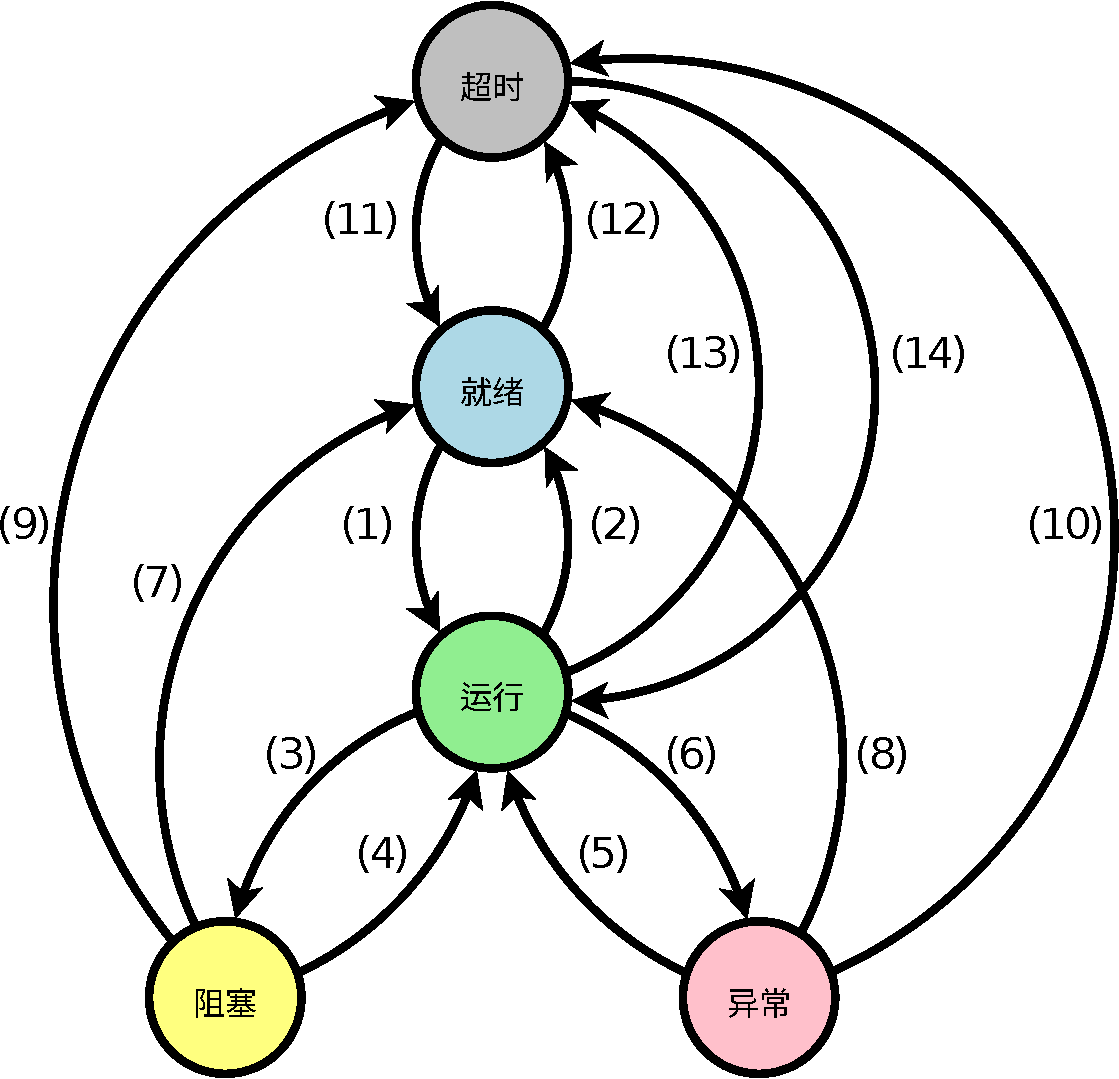
\includegraphics[width=0.72\textwidth]{Figure/image11.pdf}
    \caption{线程状态转移图}
    \label{fig:4-1-thread-state-transition-diagram}
\end{figure}

图中各个数字标号的意义如下所示：

\begin{xltabular}{\textwidth}{@{}>{\hsize=0.5279\hsize\raggedright\arraybackslash}X>{\hsize=1.4721\hsize\raggedright\arraybackslash}X@{}}
\caption{线程状态转移图中各标号的含义}\label{tab:4-7-thread-state-transition-labels}\\
\toprule
标号 & 代表意义\tabularnewline
\endfirsthead
\toprule
标号 & 代表意义\tabularnewline
\midrule
\endhead
\bottomrule
\endlastfoot
    (1) & 当前核上它是优先级最高的线程，因此由就绪态转入运行态。\tabularnewline
    (2) & 当前核上有更高优先级的线程打断了它的执行，因此由运行态转入就绪态。\tabularnewline
    (3) & 线程在一个信号端点处阻塞，因此由运行态转入阻塞态。\tabularnewline
    (4) & 线程收到了来自信号端点的信号，解除阻塞，而且是当前核上优先级最高的线程，并且其时间片没有耗尽，因此由阻塞态转入运行态。\tabularnewline
    (5) & 线程发生错误后藉由重新设置执行信息而恢复到可正常执行状态，而且是当前核上优先级最高的线程，并且其时间片没有耗尽，因此由异常态转入运行态。\tabularnewline
    (6) & 线程执行过程中发生了一个异常，因此从运行态转入异常态。\tabularnewline
    (7) & 线程收到了来自信号端点的信号，解除阻塞，并且其时间片没有耗尽，但它不是当前核上优先级最高的线程，因此由阻塞态转入就绪态。\tabularnewline
    (8) & 线程发生错误后藉由重新设置执行信息而恢复到可正常执行状态，并且其时间片没有耗尽，但它不是当前核上优先级最高的线程，因此由异常态转入就绪态。\tabularnewline
    (9) & 线程在等待信号端点时，被其他线程把自己的时间片传递出去，使得自己的时间片归零，因此在收到信号解除阻塞后由阻塞态转入超时态。\tabularnewline
    (10) & 线程发生错误后，被其他线程把自己的时间片传递出去，使得自己的时间片归零，因此在重新设置执行信息而恢复到可正常执行状态后由异常态转入超时态。\tabularnewline
    (11) & 线程被其他线程传递了时间片，重新进入可以运行的状态，但它不是当前核上优先级最高的线程，因此由超时态转入就绪态。\tabularnewline
    (12) & 线程在就绪状态时，被其他线程把自己的时间片传递出去，使得自己的时间片归零，因此由就绪态转入超时态。\tabularnewline
    (13) & 线程在运行过程中耗尽了自己的时间片，因此由运行态转入超时态。\tabularnewline
    (14) & 线程被其他线程传递了时间片，重新进入可以运行的状态，而且是当前核上优先级最高的线程，因此由超时态转入运行态。\tabularnewline
\end{xltabular}

其中，（6）（9）（10）（12）（13）等一切转入超时态和异常态的转换都会导致调度器事件的发送。

\section{进程功能列表}\label{sec:4-process-function-list}

与进程有关的内核功能如下：

\begin{xltabular}{\textwidth}{@{}>{\hsize=0.9445\hsize\raggedright\arraybackslash}X>{\hsize=0.7197\hsize\raggedright\arraybackslash}X>{\hsize=1.3358\hsize\raggedright\arraybackslash}X@{}}
\caption{进程相关内核功能}\label{tab:4-8-process-related-kernel-functions}\\
\toprule
调用号 & 类型 & 用途\tabularnewline
\endfirsthead
\toprule
调用号 & 类型 & 用途\tabularnewline
\midrule
\endhead
\bottomrule
\endlastfoot
RME\_SVC\_PRC\_CRT & 系统调用 & 创建进程\tabularnewline
RME\_SVC\_PRC\_DEL & 系统调用 & 删除进程\tabularnewline
RME\_SVC\_PRC\_CPT & 系统调用 & 替换进程的权能表\tabularnewline
RME\_SVC\_PRC\_PGT & 系统调用 &
替换进程的页表\footnote{顶层页目录}\tabularnewline
\end{xltabular}

进程权能的操作标志如下：

\begin{xltabular}{\textwidth}{@{}>{\hsize=0.9158\hsize\raggedright\arraybackslash}X>{\hsize=0.6763\hsize\raggedright\arraybackslash}X>{\hsize=1.4079\hsize\raggedright\arraybackslash}X@{}}
\caption{进程操作标志}\label{tab:4-9-process-operation-flags}\\
\toprule
标志 & 位 & 用途\tabularnewline
\endfirsthead
\toprule
标志 & 位 & 用途\tabularnewline
\midrule
\endhead
\bottomrule
\endlastfoot
RME\_PRC\_FLAG\_INV & {[}0{]} &
允许在该进程内创建同步迁移调用。\tabularnewline
RME\_PRC\_FLAG\_THD & {[}1{]} & 允许在该进程内创建线程。\tabularnewline
RME\_PRC\_FLAG\_CPT & {[}2{]} & 允许替换该进程的权能表。\tabularnewline
RME\_PRC\_FLAG\_PGT & {[}3{]} &
允许替换该进程的页表\footnote{顶层页目录}。\tabularnewline
\end{xltabular}

关于上表中的位{[}0{]}，请参见\ref{subsec:5-create-sync-invocation}
。

\subsection{创建进程}\label{subsec:4-create-a-process}

该操作会创建一个进程，并将其权能放入某个已存在的权能表。新创建的进程会引用权能表权能和页目录权能，一旦使用某对权能表/页目录权能创建了一个进程，那么这对权能在该进程被删除前就不能被移除/删除。进程权能没有单独分配的内核对象，因此不需要内核内存权能就能创建。

创建进程操作需要如下几个参数：

\begin{xltabular}{\textwidth}{@{}>{\hsize=0.7639\hsize\raggedright\arraybackslash}X>{\hsize=0.6758\hsize\raggedright\arraybackslash}X>{\hsize=0.6758\hsize\raggedright\arraybackslash}X>{\hsize=1.8846\hsize\raggedright\arraybackslash}X@{}}
\caption{创建进程的所需参数}\label{tab:4-10-create-process-parameters}\\
\toprule
参数名称 & 类型 & 域 & 描述\tabularnewline
\endfirsthead
\toprule
参数名称 & 类型 & 域 & 描述\tabularnewline
\midrule
\endhead
\bottomrule
\endlastfoot
Svc\_Num & ptr\_t & N & 必须为 RME\_SVC\_PRC\_CRT。\tabularnewline
Cap\_Cpt\_Crt & cid\_t & C &
一个对应于必须拥有 RME\_CPT\_FLAG\_CRT 属性的权能表权能的权能号，该权能号对应的权能指向要接受此新创建的进程权能的权能表。该权能号可以是一级或者二级查找编码。\tabularnewline
Cap\_Prc & cid\_t & P0 &
一个对应于接受该新创建的进程权能的权能表的某位置的权能号。该权能号对应的权能必须是空白的。该权能号只能是一级查找编码。\tabularnewline
Cap\_Cpt & cid\_t & P1 &
一个对应于必须拥有 RME\_CPT\_FLAG\_PRC\_CRT 属性的权能表权能的权能号，该权能号对应的权能指向要给新创建的进程使用的权能表。该权能号可以是一级或者二级查找编码。\tabularnewline
Cap\_Pgt & cid\_t & P2 &
一个对应于必须拥有 RME\_PGT\_FLAG\_PRC\_CRT 属性的页表权能的权能号，该权能号对应的权能指向要给新创建的进程使用的页表\footnote{顶层页目录}。该权能号可以是一级或者二级查找编码。\tabularnewline
Raw\_Pgt & ptr\_t & P2 &
一旦在移植时开启了用户态页表控制宏 RME\_PGT\_RAW\_USER，该参数即取代 Cap\_Pgt。它是处理器可直接识别的页表数据结构所在的物理地址，内核将直接使用它。因此，在使用用户态页表时，有进程创建权限的用户态进程必须可信。\tabularnewline
\end{xltabular}

该操作的返回值可能如下：

\begin{xltabular}{\textwidth}{@{}>{\hsize=0.8317\hsize\raggedright\arraybackslash}X>{\hsize=1.1683\hsize\raggedright\arraybackslash}X@{}}
\caption{创建进程的可能返回值}\label{tab:4-11-create-process-return-values}\\
\toprule
返回值 & 意义\tabularnewline
\endfirsthead
\toprule
返回值 & 意义\tabularnewline
\midrule
\endhead
\bottomrule
\endlastfoot
    0 & 操作成功。\tabularnewline
    RME\_ERR\_CPT\_RANGE & Cap\_Cpt\_Crt 的一级/二级查找超出了范围。\tabularnewline
    RME\_ERR\_CPT\_RANGE & Cap\_Cpt 的一级/二级查找超出了范围。\tabularnewline
    RME\_ERR\_CPT\_RANGE & Cap\_Pgt 的一级/二级查找超出了范围。\tabularnewline
    RME\_ERR\_CPT\_RANGE & Cap\_Prc 的一级查找超出了范围。\tabularnewline
    RME\_ERR\_CPT\_FROZEN & Cap\_Cpt\_Crt 的一级/二级查找的权能已经被冻结。\tabularnewline
    RME\_ERR\_CPT\_FROZEN & Cap\_Cpt 的一级/二级查找权能已经被冻结。\tabularnewline
    RME\_ERR\_CPT\_FROZEN & Cap\_Pgt 的一级/二级查找权能已经被冻结。\tabularnewline
    RME\_ERR\_CPT\_FROZEN & Cap\_Prc 被冻结，或者其它核正在该处创建权能。\tabularnewline
    RME\_ERR\_CPT\_TYPE & Cap\_Cpt\_Crt 或 Cap\_Cpt 不是权能表权能。\tabularnewline
    RME\_ERR\_CPT\_TYPE & Cap\_Pgt 不是页表权能。\tabularnewline
    RME\_ERR\_CPT\_FLAG & Cap\_Cpt\_Crt 无 RME\_CPT\_FLAG\_CRT 属性。\tabularnewline
    RME\_ERR\_CPT\_FLAG & Cap\_Cpt 无 RME\_CPT\_FLAG\_PRC\_CRT 属性。\tabularnewline
    RME\_ERR\_CPT\_FLAG & Cap\_Pgt 无 RME\_PGT\_FLAG\_PRC\_CRT 属性。\tabularnewline
    RME\_ERR\_CPT\_EXIST & Cap\_Prc 不是空白权能。\tabularnewline
\end{xltabular}

\subsection{删除进程}\label{subsec:4-delete-a-process}

该操作会删除一个进程。被删除的进程必须不含有线程或同步迁移调用（关于后者见同步通信机制）。删除进程需要以下几个参数：

\begin{xltabular}{\textwidth}{@{}>{\hsize=0.6910\hsize\raggedright\arraybackslash}X>{\hsize=0.6910\hsize\raggedright\arraybackslash}X>{\hsize=0.6910\hsize\raggedright\arraybackslash}X>{\hsize=1.9271\hsize\raggedright\arraybackslash}X@{}}
\caption{删除进程的所需参数}\label{tab:4-12-delete-process-parameters}\\
\toprule
参数名称 & 类型 & 域 & 描述\tabularnewline
\endfirsthead
\toprule
参数名称 & 类型 & 域 & 描述\tabularnewline
\midrule
\endhead
\bottomrule
\endlastfoot
Svc\_Num & ptr\_t & N & 必须为 RME\_SVC\_PRC\_DEL。\tabularnewline
Cap\_Cpt & cid\_t & C &
一个对应于必须拥有 RME\_CPT\_FLAG\_DEL 属性的权能表权能的权能号，该权能号对应的权能指向含有正被删除的进程权能的权能表。该权能号可以是一级或者二级查找编码。\tabularnewline
Cap\_Prc & cid\_t & P1 &
一个对应于将被删除的进程权能的权能号。该权能号对应的权能必须是一个进程权能。该权能号只能是一级查找编码。\tabularnewline
\end{xltabular}

该操作的返回值可能如下：

\begin{xltabular}{\textwidth}{@{}>{\hsize=0.6993\hsize\raggedright\arraybackslash}X>{\hsize=1.3007\hsize\raggedright\arraybackslash}X@{}}
\caption{删除进程的可能返回值}\label{tab:4-13-delete-process-return-values}\\
\toprule
返回值 & 意义\tabularnewline
\endfirsthead
\toprule
返回值 & 意义\tabularnewline
\midrule
\endhead
\bottomrule
\endlastfoot
    0 & 操作成功。\tabularnewline
    RME\_ERR\_CPT\_RANGE & Cap\_Cpt 的一级/二级查找超出了范围。\tabularnewline
    RME\_ERR\_CPT\_RANGE & Cap\_Prc 的一级查找超出了范围。\tabularnewline
    RME\_ERR\_CPT\_FROZEN & Cap\_Cpt 的一级/二级查找的权能已经被冻结。\tabularnewline
    RME\_ERR\_CPT\_FROZEN & Cap\_Prc 未被冻结。\tabularnewline
    RME\_ERR\_CPT\_TYPE & Cap\_Cpt 不是权能表权能。\tabularnewline
    RME\_ERR\_CPT\_TYPE & Cap\_Prc 不是进程权能。\tabularnewline
    RME\_ERR\_CPT\_NULL & Cap\_Prc 为空白权能。\tabularnewline
    RME\_ERR\_CPT\_NULL & 两个核同时试图删除该进程，此时未成功的核返回该值。\tabularnewline
    RME\_ERR\_CPT\_FLAG & Cap\_Cpt 无 RME\_CPT\_FLAG\_DEL 属性。\tabularnewline
    RME\_ERR\_CPT\_QUIE & Cap\_Prc 不安定。\tabularnewline
    RME\_ERR\_CPT\_REFCNT & Cap\_Prc 的引用计数不为 0，或者不为根权能\footnote{内部有线程或同步迁移调用}。\tabularnewline
\end{xltabular}

\needspace{30\baselineskip}
\subsection{更改进程的权能表}\label{subsec:4-change-process-capability-table}
\nopagebreak[4]

该操作会把进程的权能表替换成另外一个。替换完成后，立即生效。替换进程的权能表需要以下几个参数：

\begin{xltabular}{\textwidth}{@{}>{\hsize=0.6910\hsize\raggedright\arraybackslash}X>{\hsize=0.6910\hsize\raggedright\arraybackslash}X>{\hsize=0.6910\hsize\raggedright\arraybackslash}X>{\hsize=1.9271\hsize\raggedright\arraybackslash}X@{}}
\caption{更改进程权能表的所需参数}\label{tab:4-14-change-process-capability-table-parameters}\\
\toprule
参数名称 & 类型 & 域 & 描述\tabularnewline
\endfirsthead
\toprule
参数名称 & 类型 & 域 & 描述\tabularnewline
\midrule
\endhead
\bottomrule
\endlastfoot
Svc\_Num & ptr\_t & N & 必须为 RME\_SVC\_PRC\_CPT。\tabularnewline
Cap\_Prc & cid\_t & P1 &
一个对应于必须拥有 RME\_PRC\_FLAG\_CPT 属性的进程权能的权能号，该权能号对应的权能指向要修改权能表的进程。该权能号可以是一级或者二级查找编码。\tabularnewline
Cap\_Cpt & cid\_t & P2 &
一个对应于必须拥有 RME\_CPT\_FLAG\_PRC\_CPT 属性的权能表权能的权能号，该权能号对应的权能指向要给进程使用的权能表。该权能号可以是一级或者二级查找编码。\tabularnewline
\end{xltabular}

该操作的返回值可能如下：

\begin{xltabular}{\textwidth}{@{}>{\hsize=0.7784\hsize\raggedright\arraybackslash}X>{\hsize=1.2216\hsize\raggedright\arraybackslash}X@{}}
\caption{更改进程权能表的所需返回值}\label{tab:4-15-change-process-capability-table-return-values}\\
\toprule
返回值 & 意义\tabularnewline
\endfirsthead
\toprule
返回值 & 意义\tabularnewline
\midrule
\endhead
\bottomrule
\endlastfoot
    0 & 操作成功。\tabularnewline
    RME\_ERR\_CPT\_RANGE & Cap\_Prc 的一级/二级查找超出了范围。\tabularnewline
    RME\_ERR\_CPT\_RANGE & Cap\_Cpt 的一级查找超出了范围。\tabularnewline
    RME\_ERR\_CPT\_FROZEN & Cap\_Prc 的一级/二级查找的权能已经被冻结。\tabularnewline
    RME\_ERR\_CPT\_FROZEN & Cap\_Cpt 的一级/二级查找的权能已经被冻结。\tabularnewline
    RME\_ERR\_CPT\_TYPE & Cap\_Prc 不是进程权能。\tabularnewline
    RME\_ERR\_CPT\_TYPE & Cap\_Cpt 不是权能表权能。\tabularnewline
    RME\_ERR\_CPT\_NULL & Cap\_Prc 或 Cap\_Cpt 为空白权能。\tabularnewline
    RME\_ERR\_CPT\_FLAG & Cap\_Prc 无 RME\_PRC\_FLAG\_CPT 属性。\tabularnewline
    RME\_ERR\_CPT\_FLAG & Cap\_Cpt 无 RME\_CPT\_FLAG\_PRC\_CPT 属性。\tabularnewline
    RME\_ERR\_PTH\_CONFLICT & 两个核同时试图替换权能表，此时未成功的核返回该值。\tabularnewline
\end{xltabular}

\subsection{更改进程的页表}\label{subsec:4-change-process-page-table}

该操作会把进程的页表替换成另外一个。替换完成后，立即生效。替换进程的页表需要以下几个参数：

\begin{xltabular}{\textwidth}{@{}>{\hsize=0.6910\hsize\raggedright\arraybackslash}X>{\hsize=0.6910\hsize\raggedright\arraybackslash}X>{\hsize=0.6910\hsize\raggedright\arraybackslash}X>{\hsize=1.9271\hsize\raggedright\arraybackslash}X@{}}
\caption{更改进程页表的所需参数}\label{tab:4-16-change-process-page-table-parameters}\\
\toprule
参数名称 & 类型 & 域 & 描述\tabularnewline
\endfirsthead
\toprule
参数名称 & 类型 & 域 & 描述\tabularnewline
\midrule
\endhead
\bottomrule
\endlastfoot
Svc\_Num & ptr\_t & N & 必须为 RME\_SVC\_PRC\_PGT。\tabularnewline
Cap\_Prc & cid\_t & P1 &
一个对应于必须拥有 RME\_PRC\_FLAG\_PGT 属性的进程权能的权能号，该权能号对应的权能指向要修改页表\footnote{顶层页目录}的进程。该权能号可以是一级或者二级查找编码。\tabularnewline
Cap\_Pgt & cid\_t & P2 &
一个对应于必须拥有 RME\_PGT\_FLAG\_PRC\_PGT 属性的页目录权能的权能号，该权能号对应的权能指向要给进程使用的页表\footnote{顶层页目录}。该权能号可以是一级或者二级查找编码。\tabularnewline
Raw\_Pgt & ptr\_t & P2 &
一旦在移植时开启了用户态页表控制宏RME\_PGT\_RAW\_USER，该参数即取代Cap\_Pgt。它是处理器可直接识别的页表数据结构所在的物理地址，内核将直接使用它。因此，在使用用户态页表时，有本权限的用户态进程必须可信。\tabularnewline
\end{xltabular}

该操作的返回值可能如下：

\begin{xltabular}{\textwidth}{@{}>{\hsize=0.7880\hsize\raggedright\arraybackslash}X>{\hsize=1.2120\hsize\raggedright\arraybackslash}X@{}}
\caption{更改进程页表的可能返回值}\label{tab:4-17-change-process-page-table-return-values}\\
\toprule
返回值 & 意义\tabularnewline
\endfirsthead
\toprule
返回值 & 意义\tabularnewline
\midrule
\endhead
\bottomrule
\endlastfoot
    0 & 操作成功。\tabularnewline
    RME\_ERR\_CPT\_RANGE & Cap\_Prc 的一级/二级查找超出了范围。\tabularnewline
    RME\_ERR\_CPT\_RANGE & Cap\_Pgt 的一级查找超出了范围。\tabularnewline
    RME\_ERR\_CPT\_FROZEN & Cap\_Prc 的一级/二级查找的权能已经被冻结。\tabularnewline
    RME\_ERR\_CPT\_FROZEN & Cap\_Pgt 的一级/二级查找的权能已经被冻结。\tabularnewline
    RME\_ERR\_CPT\_TYPE & Cap\_Prc 不是进程权能。\tabularnewline
    RME\_ERR\_CPT\_TYPE & Cap\_Pgt 不是页表权能。\tabularnewline
    RME\_ERR\_CPT\_NULL & Cap\_Prc 或 Cap\_Pgt 为空白权能。\tabularnewline
    RME\_ERR\_CPT\_FLAG & Cap\_Prc 无 RME\_PRC\_FLAG\_PGT 属性。\tabularnewline
    RME\_ERR\_CPT\_FLAG & Cap\_Pgt 无 RME\_PGT\_FLAG\_PRC\_PGT 属性。\tabularnewline
    RME\_ERR\_PTH\_CONFLICT & 两个核同时试图替换页表，此时未成功的核返回该值。\tabularnewline
\end{xltabular}

\section{线程功能列表}\label{sec:4-thread-function-list}

与线程有关的内核功能如下：

\begin{xltabular}{\textwidth}{@{}>{\hsize=1.0550\hsize\raggedright\arraybackslash}X>{\hsize=0.6673\hsize\raggedright\arraybackslash}X>{\hsize=1.2777\hsize\raggedright\arraybackslash}X@{}}
\caption{线程相关内核功能}\label{tab:4-18-thread-related-kernel-functions}\\
\toprule
调用号 & 类型 & 用途\tabularnewline
\endfirsthead
\toprule
调用号 & 类型 & 用途\tabularnewline
\midrule
\endhead
\bottomrule
\endlastfoot
RME\_SVC\_THD\_CRT & 系统调用 & 创建线程\tabularnewline
RME\_SVC\_THD\_DEL & 系统调用 & 删除线程\tabularnewline
RME\_SVC\_THD\_SCHED\_BIND & 系统调用 & 将线程绑定到某CPU\tabularnewline
RME\_SVC\_THD\_SCHED\_FREE & 系统调用 &
将线程从某CPU上释放\footnote{顶层页目录}\tabularnewline
RME\_SVC\_THD\_EXEC\_SET & 系统调用 &
设置线程的执行属性\footnote{入口和栈}\tabularnewline
RME\_SVC\_THD\_SCHED\_PRIO & 系统调用 & 更改线程的优先级\tabularnewline
RME\_SVC\_THD\_SCHED\_RCV & 系统调用 &
收取线程的调度器事件\tabularnewline
RME\_SVC\_THD\_TIME\_XFER & 系统调用 & 在线程间传递时间片\tabularnewline
RME\_SVC\_THD\_SWT & 系统调用 & 切换到某同优先级线程\tabularnewline
\end{xltabular}

线程权能的操作标志如下：

\begin{xltabular}{\textwidth}{@{}>{\hsize=1.2600\hsize\raggedright\arraybackslash}X>{\hsize=0.5400\hsize\raggedright\arraybackslash}X>{\hsize=1.2000\hsize\raggedright\arraybackslash}X@{}}
\caption{线程操作标志}\label{tab:4-19-thread-operation-flags}\\
\toprule
标志 & 位 & 用途\tabularnewline
\endfirsthead
\toprule
标志 & 位 & 用途\tabularnewline
\midrule
\endhead
\bottomrule
\endlastfoot
RME\_THD\_FLAG\_EXEC\_SET & {[}0{]} &
允许设置该线程的执行属性。\tabularnewline
RME\_THD\_FLAG\_SCHED\_CHILD & {[}1{]} &
允许在该线程在绑定操作中作为子线程。\tabularnewline
RME\_THD\_FLAG\_SCHED\_PARENT & {[}2{]} &
允许在该线程在绑定操作中作为父线程。\tabularnewline
RME\_THD\_FLAG\_SCHED\_PRIO & {[}3{]} &
允许更改该线程的优先级。\tabularnewline
RME\_THD\_FLAG\_SCHED\_FREE & {[}4{]} &
允许解除该线程对某CPU的绑定。\tabularnewline
RME\_THD\_FLAG\_SCHED\_RCV & {[}5{]} &
允许收取该线程的调度器事件。\tabularnewline
RME\_THD\_FLAG\_XFER\_SRC & {[}6{]} &
允许该线程在时间传递中作为源。\tabularnewline
RME\_THD\_FLAG\_XFER\_DST & {[}7{]} &
允许该线程在时间传递中作为目标。\tabularnewline
RME\_THD\_FLAG\_SWT & {[}8{]} &
允许切换操作切换到该线程。\tabularnewline
\end{xltabular}

\subsection{创建线程}\label{subsec:4-create-a-thread}

该操作会创建一个线程，并将其权能放入某个已存在的权能表。新创建的线程是没有绑定到任何CPU，没有TID，并处于 RME\_THD\_TIMEOUT 状态的。为了防止一个线程新建超过自身优先级上限的线程而破坏子系统之间的隔离，任何线程都无法创建高于自身优先级上限的线程。

线程会引用创建时指定的进程，一旦使用在某进程内创建了一个线程，那么这个进程在该线程被删除前就不能被删除。考虑到部分架构中向量寄存器数量较多，本操作允许指定一个上下文属性，说明该线程允许启用的指令集，以节约内核内存的使用。本操作还允许线程映射其寄存器组到用户态；如果指定映射到用户态，则运行在用户态的虚拟机监视器可以随时修改其上下文，从而大大方便虚拟化相关功能的编程。如果内核在配置时就决定不使用虚拟化映射功能\footnote{详见第~\ref{subsec:7-general-macro-definitions}~节}，则该功能不能使用。创建线程操作需要如下几个参数：

\begin{xltabular}{\textwidth}{@{}>{\hsize=0.6786\hsize\raggedright\arraybackslash}X>{\hsize=0.6786\hsize\raggedright\arraybackslash}X>{\hsize=0.7502\hsize\raggedright\arraybackslash}X>{\hsize=1.8926\hsize\raggedright\arraybackslash}X@{}}
\caption{创建线程的所需参数}\label{tab:4-20-create-thread-parameters}\\
\toprule
参数名称 & 类型 & 域 & 描述\tabularnewline
\endfirsthead
\toprule
参数名称 & 类型 & 域 & 描述\tabularnewline
\midrule
\endhead
\bottomrule
\endlastfoot
Svc\_Num & ptr\_t & N{[}5:0{]} & 必须为 RME\_SVC\_THD\_CRT。\tabularnewline
Cap\_Cpt & cid\_t & C &
一个对应于必须拥有 RME\_CPT\_FLAG\_CRT 属性的权能表权能的权能号，该权能号对应的权能指向要接受此新创建的线程权能的权能表。该权能号可以是一级或者二级查找编码。\tabularnewline
Cap\_Kom & cid\_t & P1.D1 &
一个内核内存权能号，其标识的内核内存范围必须能够放下线程内核对象，并且要拥有 RME\_KOM\_FLAG\_THD 属性。该权能号可以是一级或二级查找编码。\tabularnewline
Cap\_Thd & cid\_t & P1.D0 &
一个对应于接受该新创建的线程权能的权能表的某位置的权能号。该权能号对应的权能必须是空白的。该权能号只能是一级查找编码。\tabularnewline
Cap\_Prc & cid\_t & P2.D1 &
一个对应于必须拥有 RME\_PRC\_FLAG\_THD 属性的进程权能的权能号，该权能号对应的权能指向包含新创建的线程的进程。该权能号可以是一级或者二级查找编码。\tabularnewline
Max\_Prio & ptr\_t & P2.D0 & 该线程的优先级上限。\tabularnewline
Raddr & ptr\_t & P3 &
新创建的线程内核对象要使用的内核起始相对虚拟地址。这个地址是相对于Cap\_Kom对应的内核权能的起始虚拟地址的。\tabularnewline
Attr & ptr\_t & N{[}X/2-1:7{]} &
指定线程的扩展指令集上下文属性。对于不同的架构，这个参数的意义不同，但在所有的架构中0都代表不进行任何指令集扩展，不分配、保存和恢复任何协处理器的寄存器状态。对于32位处理器，这个参数有9位，对于64位处理器，这个参数有25位。\tabularnewline
Is\_Hyp & ptr\_t & N{[}6{]} &
如果设置为0，系统会在内核中分配保存线程上下文的空间，这是通常情况。如果不为0，则线程将映射其寄存器到用户态，此时需要在绑定线程到CPU时设置映射的具体地址。\tabularnewline
\end{xltabular}

该操作的返回值可能如下：

\begin{xltabular}{\textwidth}{@{}>{\hsize=0.6791\hsize\raggedright\arraybackslash}X>{\hsize=1.3209\hsize\raggedright\arraybackslash}X@{}}
\caption{创建线程的可能返回值}\label{tab:4-21-create-thread-return-values}\\
\toprule
返回值 & 意义\tabularnewline
\endfirsthead
\toprule
返回值 & 意义\tabularnewline
\midrule
\endhead
\bottomrule
\endlastfoot
    0 & 操作成功。\tabularnewline
    RME\_ERR\_CPT\_RANGE & Cap\_Cpt 的一级/二级查找超出了范围。\tabularnewline
    RME\_ERR\_CPT\_RANGE & Cap\_Kom 的一级/二级查找超出了范围。\tabularnewline
    RME\_ERR\_CPT\_RANGE & Cap\_Prc 的一级/二级查找超出了范围。\tabularnewline
    RME\_ERR\_CPT\_RANGE & Cap\_Thd 的一级查找超出了范围。\tabularnewline
    RME\_ERR\_CPT\_FROZEN & Cap\_Cpt 的一级/二级查找的权能已经被冻结。\tabularnewline
    RME\_ERR\_CPT\_FROZEN & Cap\_Kom 的一级/二级查找的权能已经被冻结。\tabularnewline
    RME\_ERR\_CPT\_FROZEN & Cap\_Prc 的一级/二级查找权能已经被冻结。\tabularnewline
    RME\_ERR\_CPT\_FROZEN & Cap\_Thd 被冻结，或者其它核正在该处创建权能。\tabularnewline
    RME\_ERR\_CPT\_TYPE & Cap\_Cpt 不是权能表权能。\tabularnewline
    RME\_ERR\_CPT\_TYPE & Cap\_Kom 不是内核内存权能。\tabularnewline
    RME\_ERR\_CPT\_TYPE & Cap\_Prc 不是进程权能。\tabularnewline
    RME\_ERR\_CPT\_FLAG & Cap\_Cpt 无 RME\_CPT\_FLAG\_CRT 属性。\tabularnewline
    RME\_ERR\_CPT\_FLAG & Cap\_Kom 无 RME\_KOM\_FLAG\_THD 属性，或范围错误。\tabularnewline
    RME\_ERR\_CPT\_FLAG & Cap\_Prc 无 RME\_PRC\_FLAG\_THD 属性。\tabularnewline
    RME\_ERR\_CPT\_EXIST & Cap\_Thd 不是空白权能。\tabularnewline
    RME\_ERR\_CPT\_KOT & 分配内核内存失败。\tabularnewline
    RME\_ERR\_PTH\_PRIO & 试图创建比自身拥有更高的优先级上限的线程，或者传入的优先级上限过大，超过了系统配置时允许的上限。\tabularnewline
\bottomrule
\end{xltabular}

\needspace{30\baselineskip}
\subsection{删除线程}\label{subsec:4-delete-a-thread}
\nopagebreak[4]

该操作会删除一个线程。被删除的线程必须已经被解除绑定。删除线程需要以下几个参数：

\begin{xltabular}{\textwidth}{@{}>{\hsize=0.6910\hsize\raggedright\arraybackslash}X>{\hsize=0.6910\hsize\raggedright\arraybackslash}X>{\hsize=0.6910\hsize\raggedright\arraybackslash}X>{\hsize=1.9271\hsize\raggedright\arraybackslash}X@{}}
\caption{删除线程的所需参数}\label{tab:4-22-delete-thread-parameters}\\
\toprule
参数名称 & 类型 & 域 & 描述\tabularnewline
\endfirsthead
\toprule
参数名称 & 类型 & 域 & 描述\tabularnewline
\midrule
\endhead
Svc\_Num & ptr\_t & N & 必须为 RME\_SVC\_THD\_DEL。\tabularnewline
Cap\_Cpt & cid\_t & C &
一个对应于必须拥有 RME\_CPT\_FLAG\_DEL 属性的权能表权能的权能号，该权能号对应的权能指向含有正被删除的线程权能的权能表。该权能号可以是一级或者二级查找编码。\tabularnewline
Cap\_Thd & cid\_t & P1 &
一个对应于将被删除的线程权能的权能号。该权能号对应的权能必须是一个线程权能。该权能号只能是一级查找编码。\tabularnewline
\end{xltabular}

该操作的返回值可能如下：

\begin{xltabular}{\textwidth}{@{}>{\hsize=0.7784\hsize\raggedright\arraybackslash}X>{\hsize=1.2216\hsize\raggedright\arraybackslash}X@{}}
\caption{删除线程的可能返回值}\label{tab:4-23-delete-thread-return-values}\\
\toprule
返回值 & 意义\tabularnewline
\endfirsthead
\toprule
返回值 & 意义\tabularnewline
\midrule
\endhead
\bottomrule
\endlastfoot
    0 & 操作成功。\tabularnewline
    RME\_ERR\_CPT\_RANGE & Cap\_Cpt 的一级/二级查找超出了范围。\tabularnewline
    RME\_ERR\_CPT\_RANGE & Cap\_Thd 的一级查找超出了范围。\tabularnewline
    RME\_ERR\_CPT\_FROZEN & Cap\_Cpt 的一级/二级查找的权能已经被冻结。\tabularnewline
    RME\_ERR\_CPT\_FROZEN & Cap\_Thd 未被冻结。\tabularnewline
    RME\_ERR\_CPT\_TYPE & Cap\_Cpt 不是权能表权能。\tabularnewline
    RME\_ERR\_CPT\_TYPE & Cap\_Thd 不是线程权能。\tabularnewline
    RME\_ERR\_CPT\_NULL & Cap\_Thd 为空白权能。\tabularnewline
    RME\_ERR\_CPT\_NULL & 两个核同时试图删除该线程，此时未成功的核返回该值。\tabularnewline
    RME\_ERR\_CPT\_FLAG & Cap\_Cpt 无 RME\_CPT\_FLAG\_DEL 属性。\tabularnewline
    RME\_ERR\_CPT\_QUIE & Cap\_Thd 不安定。\tabularnewline
    RME\_ERR\_CPT\_REFCNT & Cap\_Thd 的引用计数不为 0，或者不为根权能。\tabularnewline
    RME\_ERR\_PTH\_INVSTATE & 该线程仍然处于被绑定状态。\tabularnewline
\end{xltabular}

\subsection{将线程绑定到某CPU}\label{subsec:4-bind-a-thread-to-a-cpu}

该操作会将线程绑定到某CPU上。被设置的线程必须未被绑定于任何CPU。在哪个CPU上调用本函数，绑定就完成在哪个CPU上。对于那些希望将寄存器上下文映射到用户态以方便修改的线程，该操作还会设置上下文的映射地址：对这段地址的管理由用户态下的受信任守护进程全权负责，内核在启动时只保证这个地址既可以由内核态访问，也可以由用户态访问，且不会导致缺页中断。将线程绑定到某CPU需要以下几个参数：

\begin{xltabular}{\textwidth}{@{}>{\hsize=0.8146\hsize\raggedright\arraybackslash}X>{\hsize=0.6652\hsize\raggedright\arraybackslash}X>{\hsize=0.6652\hsize\raggedright\arraybackslash}X>{\hsize=1.8550\hsize\raggedright\arraybackslash}X@{}}
\caption{将线程绑定到某CPU的所需参数}\label{tab:4-24-bind-thread-to-cpu-parameters}\\
\toprule
参数名称 & 类型 & 域 & 描述\tabularnewline
\endfirsthead
\toprule
参数名称 & 类型 & 域 & 描述\tabularnewline
\midrule
\endhead
\bottomrule
\endlastfoot
Svc\_Num & ptr\_t & N & 必须为 RME\_SVC\_THD\_SCHED\_BIND。\tabularnewline
Cap\_Thd & cid\_t & C &
一个对应于必须拥有 RME\_THD\_FLAG\_SCHED\_CHILD 属性的线程权能的权能号，该权能号对应的权能指向被绑定的线程。该权能号可以是一级或者二级查找编码。\tabularnewline
Cap\_Thd\_Sched & cid\_t & P1.D1 &
一个对应于必须拥有 RME\_THD\_FLAG\_SCHED\_PARENT 属性的线程权能的权能号，该权能号对应的权能指向被绑定的线程的父线程。该父线程必须已经被绑定于调用本函数的CPU。该权能号可以是一级或者二级查找编码。\tabularnewline
Cap\_Sig & cid\_t & P1.D0 &
一个对应于必须拥有 RME\_SIG\_FLAG\_SCHED 属性的信号端点权能的权能号。当调度器事件发生\footnote{线程超时或错误，其中超时可能由线程在运行时消耗所有时间片或者其时间片完全被传递给其他线程所致}时，该端点会收到一个信号。该权能号可以是一级或者二级查找编码，而且也是可选的。如果不希望接收调度器信号，则可以传入 RME\_CID\_NULL\footnote{一个半字长 INT\_MIN（负值），在 32 位系统上为 0x8000，在 64 位系统上为 0x80000000}。\tabularnewline
TID & tid\_t & P2.D1 &
用户提供的TID。RME 本身并不检查系统中是否有两个线程拥有相同的ID；至于是否要做这种检查是用户态的事情。\tabularnewline
Prio & ptr\_t & P2.D0 &
被绑定的线程的抢占优先级。在 RME 中线程的优先级从0开始计算，值越大优先级越高。这个值不能超过该线程固有的优先级上限。\tabularnewline
Haddr & ptr\_t & P3 &
用户态寄存器上下文的映射地址。这个地址必须位于系统中专门用于线程上下文映射的地址范围，也即大于或等于基地址RME\_HYP\_VA\_BASE，小于结束地址RME\_HYP\_VA\_BASE+
RME\_HYP\_SIZE，而且要对齐到字。对于常规的线程，设置为NULL即可。\tabularnewline
\end{xltabular}

该操作的返回值可能如下：

\begin{xltabular}{\textwidth}{@{}>{\hsize=0.7880\hsize\raggedright\arraybackslash}X>{\hsize=1.2120\hsize\raggedright\arraybackslash}X@{}}
\caption{将线程绑定到某CPU的可能返回值}\label{tab:4-25-bind-thread-to-cpu-return-values}\\
\toprule
返回值 & 意义\tabularnewline
\endfirsthead
\toprule
返回值 & 意义\tabularnewline
\midrule
\endhead
\bottomrule
\endlastfoot
    0 & 操作成功。\tabularnewline
    RME\_ERR\_CPT\_RANGE & Cap\_Thd 或 Cap\_Thd\_Sched 的一级/二级查找超出了范围。\tabularnewline
    RME\_ERR\_CPT\_FROZEN & Cap\_Thd 或 Cap\_Thd\_Sched 的一级/二级查找的权能已经被冻结。\tabularnewline
    RME\_ERR\_CPT\_TYPE & Cap\_Thd 或 Cap\_Thd\_Sched 不是线程权能，或者为空白权能。\tabularnewline
    RME\_ERR\_CPT\_FLAG & Cap\_Thd 无 RME\_THD\_FLAG\_SCHED\_CHILD 属性。\tabularnewline
    RME\_ERR\_CPT\_FLAG & Cap\_Thd\_Sched 无 RME\_THD\_FLAG\_SCHED\_PARENT 属性。\tabularnewline
    RME\_ERR\_CPT\_FLAG & 当传入 Cap\_Sig 时，它没有 RME\_SIG\_FLAG\_SCHED 属性。\tabularnewline
    RME\_ERR\_CPT\_FLAG & 欲绑定的处理器不支持该线程创建时登记的 Attr。\tabularnewline
    RME\_ERR\_PTH\_HADDR & 传入的Haddr不在系统允许范围内，不合法。\tabularnewline
    RME\_ERR\_PTH\_NOTIF & 试图注册自己为自己的父线程，不合法。\tabularnewline
    RME\_ERR\_PTH\_PRIO & 抢占优先级超过了该线程固有的优先级上限，不合法。\tabularnewline
    RME\_ERR\_PTH\_INVSTATE & Cap\_Thd 处于被绑定状态或 Cap\_Thd\_Sched 处于未被绑定状态。\tabularnewline
    RME\_ERR\_PTH\_INVSTATE & Cap\_Thd\_Sched 被绑定到了和调用本函数的 CPU 不同的 CPU。\tabularnewline
    RME\_ERR\_PTH\_CONFLICT & 如果两个CPU同时尝试绑定，在失败的CPU上返回该值。\tabularnewline
\end{xltabular}

\subsection{解除线程对某CPU的绑定}\label{subsec:4-unbind-a-thread-from-a-cpu}

该操作会解除线程对某个CPU的绑定。被解除绑定的线程自身不能有子线程。如果被解除绑定的线程向其父线程发送了调度器事件，那么这个事件会被撤销。如果被解除绑定的线程阻塞，那么它同时会让这次阻塞接收强制结束并返回RME\_ERR\_SIV\_FREE。解除线程对某CPU的绑定需要以下几个参数：

\begin{xltabular}{\textwidth}{@{}>{\hsize=0.6910\hsize\raggedright\arraybackslash}X>{\hsize=0.6910\hsize\raggedright\arraybackslash}X>{\hsize=0.6910\hsize\raggedright\arraybackslash}X>{\hsize=1.9271\hsize\raggedright\arraybackslash}X@{}}
\caption{解除线程对某CPU绑定的所需参数}\label{tab:4-26-unbind-thread-from-cpu-parameters}\\
\toprule
参数名称 & 类型 & 域 & 描述\tabularnewline
\endfirsthead
\toprule
参数名称 & 类型 & 域 & 描述\tabularnewline
\midrule
\endhead
\bottomrule
\endlastfoot
Svc\_Num & ptr\_t & N &
必须为RME\_SVC\_THD\_SCHED\_FREE。\tabularnewline
Cap\_Thd & cid\_t & P1 &
一个对应于必须拥有RME\_THD\_FLAG\_SCHED\_FREE属性的线程权能的权能号，该权能号对应的权能指向要解除绑定的线程。该权能号可以是一级或者二级查找编码。\tabularnewline
\end{xltabular}

该操作的返回值可能如下：

\begin{xltabular}{\textwidth}{@{}>{\hsize=0.7905\hsize\raggedright\arraybackslash}X>{\hsize=1.2095\hsize\raggedright\arraybackslash}X@{}}
\caption{解除线程对某CPU绑定的可能返回值}\label{tab:4-27-unbind-thread-from-cpu-return-values}\\
\toprule
返回值 & 意义\tabularnewline
\endfirsthead
\toprule
返回值 & 意义\tabularnewline
\midrule
\endhead
\bottomrule
\endlastfoot
    0 & 操作成功。\tabularnewline
    RME\_ERR\_CPT\_RANGE & Cap\_Thd的一级/二级查找超出了范围。\tabularnewline
    RME\_ERR\_CPT\_FROZEN & Cap\_Thd的一级/二级查找的权能已经被冻结。\tabularnewline
    RME\_ERR\_CPT\_TYPE & Cap\_Thd 不是线程权能，或者为空白权能。\tabularnewline
    RME\_ERR\_CPT\_FLAG & Cap\_Thd无RME\_THD\_FLAG\_SCHED\_FREE属性。\tabularnewline
    RME\_ERR\_PTH\_REFCNT & Cap\_Thd 仍然是某些线程的父线程\footnote{调度器线程}。\tabularnewline
    RME\_ERR\_PTH\_INVSTATE & Cap\_Thd处于未被绑定状态。\tabularnewline
    RME\_ERR\_PTH\_INVSTATE & Cap\_Thd被绑定到了和调用本函数的CPU不同的CPU。\tabularnewline
\end{xltabular}

\subsection{设置线程执行属性}\label{subsec:4-set-thread-execution-attributes}

该操作会设置线程的执行属性，也即其入口，栈和参数。被设置的线程必须已经被绑定于某个CPU，而且设置执行属性必须在这个CPU上进行。对于一个已经处于RME\_THD\_EXCPEND状态的线程，设置线程执行属性会视其现有时间片数将其置为RME\_THD\_READY或RME\_THD\_TIMEOUT状态，其中后者会发送一个调度器事件。当传入的Entry和Stack均为NULL时，该线程的执行属性不变，仅仅会更改其状态，这在异常处理中是很有用的。设置线程执行属性需要以下几个参数：

\begin{xltabular}{\textwidth}{@{}>{\hsize=0.6910\hsize\raggedright\arraybackslash}X>{\hsize=0.6910\hsize\raggedright\arraybackslash}X>{\hsize=0.6910\hsize\raggedright\arraybackslash}X>{\hsize=1.9271\hsize\raggedright\arraybackslash}X@{}}
\caption{设置线程执行属性的所需参数}\label{tab:4-28-set-thread-execution-attributes-parameters}\\
\toprule
参数名称 & 类型 & 域 & 描述\tabularnewline
\endfirsthead
\toprule
参数名称 & 类型 & 域 & 描述\tabularnewline
\midrule
\endhead
\bottomrule
\endlastfoot
Svc\_Num & ptr\_t & N & 必须为RME\_SVC\_THD\_EXEC\_SET。\tabularnewline
Cap\_Thd & cid\_t & C &
一个对应于必须拥有RME\_THD\_FLAG\_EXEC\_SET属性的线程权能的权能号，该权能号对应的权能指向被设置执行属性的线程。该权能号可以是一级或者二级查找编码。\tabularnewline
Entry & ptr\_t & P1 &
该线程的入口。这个值是该线程所在的进程内部的一个虚拟地址，线程将从这里开始执行。如果传入NULL，则不做任何实际改动。\tabularnewline
Stack & ptr\_t & P2 &
该线程的执行栈。这个值是该线程所在的进程内部的一个虚拟地址，线程将使用这个地址作为栈的起始。具体的栈是递增堆栈还是递减堆栈由用户态库决定。如果传入NULL，则不做任何实际改动。\tabularnewline
Param & ptr\_t & P3 & 要传递给该线程的参数。\tabularnewline
\end{xltabular}

该操作的返回值可能如下：

\begin{xltabular}{\textwidth}{@{}>{\hsize=0.8314\hsize\raggedright\arraybackslash}X>{\hsize=1.1686\hsize\raggedright\arraybackslash}X@{}}
\caption{设置线程执行属性的可能返回值}\label{tab:4-29-set-thread-execution-attributes-return-values}\\
\toprule
返回值 & 意义\tabularnewline
\endfirsthead
\toprule
返回值 & 意义\tabularnewline
\midrule
\endhead
\bottomrule
\endlastfoot
    0 & 操作成功。\tabularnewline
    RME\_ERR\_CPT\_RANGE & Cap\_Thd的一级/二级查找超出了范围。\tabularnewline
    RME\_ERR\_CPT\_FROZEN & Cap\_Thd的一级/二级查找的权能已经被冻结。\tabularnewline
    RME\_ERR\_CPT\_TYPE & Cap\_Thd 不是线程权能，或者为空白权能。\tabularnewline
    RME\_ERR\_CPT\_FLAG & Cap\_Thd无RME\_THD\_FLAG\_EXEC\_SET属性。\tabularnewline
    RME\_ERR\_PTH\_INVSTATE & 线程处于未被绑定状态。\tabularnewline
\end{xltabular}

\subsection{更改线程优先级}\label{subsec:4-change-thread-priority}

该操作会一次性更改最多四个已经绑定到某CPU的线程的优先级。当指定多于一个线程时，这些优先级更改操作是事务性（Transactional）的：它们要么全部成功，要么全部失败。当指定少于四个线程时，用不到的参数可以不填充。所有更改优先级的操作必须在同一个CPU上进行。更改线程优先级需要以下几个参数：

\begin{xltabular}{\textwidth}{@{}>{\hsize=0.6910\hsize\raggedright\arraybackslash}X>{\hsize=0.6910\hsize\raggedright\arraybackslash}X>{\hsize=0.6910\hsize\raggedright\arraybackslash}X>{\hsize=1.9271\hsize\raggedright\arraybackslash}X@{}}
\caption{更改线程优先级的所需参数}\label{tab:4-30-change-thread-priority-parameters}\\
\toprule
参数名称 & 类型 & 域 & 描述\tabularnewline
\endfirsthead
\toprule
参数名称 & 类型 & 域 & 描述\tabularnewline
\midrule
\endhead
\bottomrule
\endlastfoot
Svc\_Num & ptr\_t & N & 必须为 RME\_SVC\_THD\_SCHED\_PRIO。\tabularnewline
Number & ptr\_t & C &
指定需要修改优先级的线程的个数，允许值为1\textasciitilde4。\tabularnewline
Cap\_Thd0 & cid\_t & P1.D0 &
一个对应于必须拥有 RME\_THD\_FLAG\_SCHED\_PRIO 属性的线程权能的权能号，该权能号对应的权能指向要修改抢占优先级的线程。该权能号可以是一级或者二级查找编码。\tabularnewline
Prio0 & ptr\_t & P3.Q0 &
线程的新的抢占优先级。在 RME 中线程的优先级从0开始计算，值越大优先级越高。这个值不能超过该线程固有的优先级上限。\tabularnewline
Cap\_Thd1 & cid\_t & P1.D1 & 第二个线程（可选）的权能号。\tabularnewline
Prio1 & ptr\_t & P3.Q1 &
第二个线程（可选）的新的抢占优先级。\tabularnewline
Cap\_Thd2 & cid\_t & P2.D0 & 第三个线程（可选）的权能号。\tabularnewline
Prio2 & ptr\_t & P3.Q2 &
第三个线程（可选）的新的抢占优先级。\tabularnewline
Cap\_Thd3 & cid\_t & P2.D1 & 第四个线程（可选）的权能号。\tabularnewline
Prio3 & ptr\_t & P3.Q3 &
第四个线程（可选）的新的抢占优先级。\tabularnewline
\end{xltabular}

该操作的返回值可能如下：

\begin{xltabular}{\textwidth}{@{}>{\hsize=0.7437\hsize\raggedright\arraybackslash}X>{\hsize=1.2563\hsize\raggedright\arraybackslash}X@{}}
\caption{更改线程优先级的可能返回值}\label{tab:4-31-change-thread-priority-return-values}\\
\toprule
返回值 & 意义\tabularnewline
\endfirsthead
\toprule
返回值 & 意义\tabularnewline
\midrule
\endhead
\bottomrule
\endlastfoot
    0 & 操作成功。\tabularnewline
    RME\_ERR\_CPT\_RANGE & 四个 Cap\_Thd 中至少一个的一级/二级查找超出了范围。\tabularnewline
    RME\_ERR\_CPT\_FROZEN & 四个 Cap\_Thd 中至少一个的一级/二级查找的权能已经被冻结。\tabularnewline
    RME\_ERR\_CPT\_TYPE & 四个 Cap\_Thd 中至少一个不是线程权能，或者为空白权能。\tabularnewline
    RME\_ERR\_CPT\_FLAG & 四个 Cap\_Thd 中至少一个无 RME\_THD\_FLAG\_SCHED\_PRIO 属性。\tabularnewline
    RME\_ERR\_PTH\_PRIO & 至少一个线程的优先级超过了该线程固有的优先级上限，不合法。\tabularnewline
    RME\_ERR\_PTH\_PRIO & Number 的数值不在 1~4 之间。\tabularnewline
    RME\_ERR\_PTH\_INVSTATE & 至少一个线程处于未被绑定状态。\tabularnewline
    RME\_ERR\_PTH\_INVSTATE & 至少一个线程被绑定到了和调用本函数的CPU不同的CPU。\tabularnewline
\end{xltabular}

\needspace{30\baselineskip}
\subsection{接收线程的调度器事件}\label{subsec:4-receive-thread-scheduler-event}
\nopagebreak[4]

该操作会接收一个线程的调度器事件。该操作不会阻塞，如果该线程暂时没有调度器事件，那么我们返回一个负值。返回的值如果为正，则它可能由异常标识符 RME\_THD\_EXCPEND\_FLAG\footnote{倒数第二个二进制位}、时间片耗尽标识符 RME\_THD\_TIMEOUT\_FLAG\footnote{倒数第三个二进制位}和线程标识符 TID\footnote{其他后续二进制位}三部分组成。

RME\_THD\_EXCPEND\_FLAG置位说明线程处于异常态，此时可以利用\ref{subsec:8-get-thread-exception-register-set}
所述的内核功能调用查询异常原因，并利用RME\_SVC\_THD\_EXEC\_SET排除异常继续执行；RME\_THD\_TIMEOUT\_FLAG置位说明线程处于超时态，此时可以利用RME\_SVC\_THD\_TIME\_XFER传递更多时间片给它。这两个标识符可以同时存在：当它们同时存在时说明线程处于异常态且持有时间片为0，一旦设置其执行属性以清除其异常态后线程会立刻进入超时态\footnote{此次由异常态到超时态的转换也会发送调度器事件}。

接收一个线程的调度器事件需要如下参数：

\begin{xltabular}{\textwidth}{@{}>{\hsize=0.6910\hsize\raggedright\arraybackslash}X>{\hsize=0.6910\hsize\raggedright\arraybackslash}X>{\hsize=0.6910\hsize\raggedright\arraybackslash}X>{\hsize=1.9271\hsize\raggedright\arraybackslash}X@{}}
\caption{接收线程调度器事件的所需参数}\label{tab:4-32-receive-thread-scheduler-event-parameters}\\
\toprule
参数名称 & 类型 & 域 & 描述\tabularnewline
\endfirsthead
\toprule
参数名称 & 类型 & 域 & 描述\tabularnewline
\midrule
\endhead
\bottomrule
\endlastfoot
Svc\_Num & ptr\_t & N & 必须为 RME\_SVC\_THD\_SCHED\_RCV。\tabularnewline
Cap\_Thd & cid\_t & P1 &
一个对应于必须拥有 RME\_THD\_FLAG\_SCHED\_RCV 属性的线程权能的权能号，我们试图接收该线程的子线程发来的调度器事件。该权能号可以是一级或者二级查找编码。\tabularnewline
\end{xltabular}

该操作的返回值可能如下：

\begin{xltabular}{\textwidth}{@{}>{\hsize=0.7023\hsize\raggedright\arraybackslash}X>{\hsize=1.2977\hsize\raggedright\arraybackslash}X@{}}
\caption{接收线程调度器事件的可能返回值}\label{tab:4-33-receive-thread-scheduler-event-return-values}\\
\toprule
返回值 & 意义\tabularnewline
\endfirsthead
\toprule
返回值 & 意义\tabularnewline
\midrule
\endhead
\bottomrule
\endlastfoot
    非负值 & 操作成功。如果错误标识符为 0，那么接收到的是线程超时事件，表明线程标识符对应的线程耗尽了时间片而停止执行。如果错误标识符为 1，那么表明线程标识符对应的线程在执行中发生了一个错误，被迫停止执行。\tabularnewline
    RME\_ERR\_CPT\_RANGE & Cap\_Thd 的一级/二级查找超出了范围。\tabularnewline
    RME\_ERR\_CPT\_FROZEN & Cap\_Thd 的一级/二级查找的权能已经被冻结。\tabularnewline
    RME\_ERR\_CPT\_TYPE & Cap\_Thd 不是线程权能，或者为空白权能。\tabularnewline
    RME\_ERR\_CPT\_FLAG & Cap\_Thd 无 RME\_THD\_FLAG\_SCHED\_RCV 属性。\tabularnewline
    RME\_ERR\_PTH\_NOTIF & Cap\_Thd 暂无调度器事件可以接收。\tabularnewline
    RME\_ERR\_PTH\_INVSTATE & Cap\_Thd 处于未被绑定状态。\tabularnewline
    RME\_ERR\_PTH\_INVSTATE & Cap\_Thd 被绑定到了和调用本函数的 CPU 不同的 CPU。\tabularnewline
\end{xltabular}

\subsection{在线程间传递运行时间片}\label{subsec:4-transfer-run-time-slice-between-threads}

该操作被用来在线程之间传递时间片。时间片的源线程\footnote{源线程}和目标线程\footnote{目标线程}必须被绑定于同一个CPU上，而且本系统调用必须在这个CPU上进行，以保证传递的时间是该CPU上的执行时间。源线程本身持有的时间片和传递的时间片必须不为0。若源线程在传递时失去其所有时间片，会立即向其调度器线程发送调度器事件。

该函数允许低优先级线程给高优先级线程传递运行时间片，但不允许低优先级上限线程给高优先级上限线程\footnote{除了 Init 线程以外的；作为一种特殊情况，传递时间片给 Init 线程来作废时间是允许的}传递运行时间片：这是为了保证时间片在传递过程中总是劣化（Degrade），不至于使低优先级子系统干扰高优先级子系统。

传递运行时间片需要以下几个参数：

\begin{xltabular}{\textwidth}{@{}>{\hsize=0.7639\hsize\raggedright\arraybackslash}X>{\hsize=0.6758\hsize\raggedright\arraybackslash}X>{\hsize=0.6758\hsize\raggedright\arraybackslash}X>{\hsize=1.8846\hsize\raggedright\arraybackslash}X@{}}
\caption{在线程间传递运行时间片的所需参数}\label{tab:4-34-transfer-run-time-slice-between-threads-parameters}\\
\toprule
参数名称 & 类型 & 域 & 描述\tabularnewline
\endfirsthead
\toprule
参数名称 & 类型 & 域 & 描述\tabularnewline
\midrule
\endhead
\bottomrule
\endlastfoot
Svc\_Num & ptr\_t & N & 必须为 RME\_SVC\_THD\_TIME\_XFER。\tabularnewline
Cap\_Thd\_Dst & cid\_t & P1 &
一个对应于必须拥有 RME\_THD\_FLAG\_XFER\_DST 属性的线程权能的权能号，该权能号对应的权能指向目标线程。该权能号可以是一级或者二级查找编码。\tabularnewline
Cap\_Thd\_Src & cid\_t & P2 &
一个对应于必须拥有 RME\_THD\_FLAG\_XFER\_SRC 属性的线程权能的权能号，该权能号对应的权能指向源线程。该权能号可以是一级或者二级查找编码。\tabularnewline
Time\strut
 & ptr\_t\strut
 & P3\strut
 & 要传递的时间片数量。这个值的单位是时间片，单个时间片的大小在系统编译时被决定。该值不能为0。

传入 RME\_THD\_INF\_TIME 进行无限传递。

传入 RME\_THD\_INIT\_TIME 进行回收传递。

传入其它非0值进行普通传递。\strut
\tabularnewline
\end{xltabular}

该操作的返回值可能如下：

\begin{xltabular}{\textwidth}{@{}>{\hsize=1.0000\hsize\raggedright\arraybackslash}X>{\hsize=1.0000\hsize\raggedright\arraybackslash}X@{}}
\caption{在线程间传递运行时间片的可能返回值}\label{tab:4-35-transfer-run-time-slice-between-threads-return-values}\\
\toprule
返回值 & 意义\tabularnewline
\endfirsthead
\toprule
返回值 & 意义\tabularnewline
\midrule
\endhead
\bottomrule
\endlastfoot
    非负值 & 操作成功，返回的是目标线程现有的时间片数。如果是进行无限传递和回收传递且目标线程变成了无限线程，那么返回 RME\_THD\_INF\_TIME。\tabularnewline
    RME\_ERR\_CPT\_RANGE & Cap\_Thd\_Dst 或 Cap\_Thd\_Src 的一级/二级查找超出了范围。\tabularnewline
    RME\_ERR\_CPT\_FROZEN & Cap\_Thd\_Dst 或 Cap\_Thd\_Src 的一级/二级查找的权能已经被冻结。\tabularnewline
    RME\_ERR\_CPT\_TYPE & Cap\_Thd\_Dst 或 Cap\_Thd\_Src 不是线程权能，或者为空白权能。\tabularnewline
    RME\_ERR\_CPT\_FLAG & Cap\_Thd\_Dst 无 RME\_THD\_FLAG\_XFER\_DST 属性。\tabularnewline
    RME\_ERR\_CPT\_FLAG & Cap\_Thd\_Src 无 RME\_THD\_FLAG\_XFER\_SRC 属性。\tabularnewline
    RME\_ERR\_PTH\_INVSTATE & Cap\_Thd\_Src 无时间片可传递。\tabularnewline
    RME\_ERR\_PTH\_INVSTATE & Cap\_Thd\_Dst 或 Cap\_Thd\_Src 处于未被绑定状态。\tabularnewline
    RME\_ERR\_PTH\_INVSTATE & Cap\_Thd\_Dst 或 Cap\_Thd\_Src 被绑定到了和调用本函数的 CPU 不同的 CPU。\tabularnewline
    RME\_ERR\_PTH\_PRIO & Cap\_Thd\_Dst 的优先级上限比 Cap\_Thd\_Src 要高，而且 Cap\_Thd\_Dst 不是一个初始线程。\tabularnewline
    RME\_ERR\_PTH\_OVERFLOW & 接收该时间片的线程的时间片已满。这个错误是很罕见的，因为一般传递的时间片达不到该值\footnote{再接收的话就会超过或等于系统允许的最大值 RME\_THD\_INF\_TIME}。\tabularnewline
\end{xltabular}

\needspace{30\baselineskip}
\subsection{切换到某线程}\label{subsec:4-switch-to-a-thread}
\nopagebreak[4]

该操作允许用户态调度器直接切换到某个绑定于同一CPU上的线程，方便用户态调度的实现。被切换到的线程必须和当前线程的优先级相同，而且必须处于就绪（RME\_THD\_READY）状态。要进行线程切换，需要如下参数：

\begin{xltabular}{\textwidth}{@{}>{\hsize=0.6910\hsize\raggedright\arraybackslash}X>{\hsize=0.6910\hsize\raggedright\arraybackslash}X>{\hsize=0.6910\hsize\raggedright\arraybackslash}X>{\hsize=1.9271\hsize\raggedright\arraybackslash}X@{}}
\caption{切换到某线程的所需参数}\label{tab:4-36-switch-to-thread-parameters}\\
\toprule
参数名称 & 类型 & 域 & 描述\tabularnewline
\endfirsthead
\toprule
参数名称 & 类型 & 域 & 描述\tabularnewline
\midrule
\endhead
\bottomrule
\endlastfoot
Svc\_Num & ptr\_t & N & 必须为 RME\_SVC\_THD\_SWT。\tabularnewline
Cap\_Thd & cid\_t & P1 &
一个对应于必须拥有 RME\_THD\_FLAG\_SWT 属性的线程权能的权能号，该权能号对应的权能指向要切换到的线程。该权能号可以是一级或者二级查找编码。如果不想指定要切换的线程，而要内核决定，那么可以传入 RME\_CID\_NULL\footnote{一个半字长 INT\_MIN（负值），在 32 位系统上为 0x8000，在 64 位系统上为 0x80000000}。\tabularnewline
Is\_Yield & ptr\_t & P2 &
此次线程切换是否放弃当前线程的全部时间片。如果该项不为0，那么此次切换会放弃当前线程的全部时间片，并立即向其调度器线程发送调度器事件。如果是在 Init 线程或无限线程中调用，那么该项无效，因为 Init 线程或无限线程的时间片是无限的。\tabularnewline
\end{xltabular}

\needspace{20\baselineskip}
该操作的返回值可能如下：

\begin{xltabular}{\textwidth}{@{}>{\hsize=0.8626\hsize\raggedright\arraybackslash}X>{\hsize=1.1374\hsize\raggedright\arraybackslash}X@{}}
\caption{切换到某线程的可能返回值}\label{tab:4-37-switch-to-thread-return-values}\\
\toprule
返回值 & 意义\tabularnewline
\endfirsthead
\toprule
返回值 & 意义\tabularnewline
\midrule
\endhead
\bottomrule
\endlastfoot
    0 & 操作成功。\tabularnewline
    RME\_ERR\_CPT\_RANGE & Cap\_Thd 的一级/二级查找超出了范围。\tabularnewline
    RME\_ERR\_CPT\_FROZEN & Cap\_Thd 的一级/二级查找的权能已经被冻结。\tabularnewline
    RME\_ERR\_CPT\_TYPE & Cap\_Thd 不是线程权能，或者为空白权能。\tabularnewline
    RME\_ERR\_CPT\_FLAG & Cap\_Thd 无 RME\_THD\_FLAG\_SWT 属性。\tabularnewline
    RME\_ERR\_PTH\_INVSTATE & Cap\_Thd 处于未被绑定状态。\tabularnewline
    RME\_ERR\_PTH\_INVSTATE & Cap\_Thd 被绑定到了和调用本函数的 CPU 不同的 CPU。\tabularnewline
    RME\_ERR\_PTH\_INVSTATE & Cap\_Thd 处于阻塞（RME\_THD\_BLOCKED）状态。\tabularnewline
    RME\_ERR\_PTH\_INVSTATE & Cap\_Thd 处于超时（RME\_THD\_TIMEOUT）状态。\tabularnewline
    RME\_ERR\_PTH\_INVSTATE & Cap\_Thd 处于异常（RME\_THD\_EXCPEND）状态。\tabularnewline
    RME\_ERR\_PTH\_PRIO & Cap\_Thd 的优先级和当前线程的优先级不同。\tabularnewline
\end{xltabular}

\section{本章参考文献}\label{sec:4-chapter-bibliography}

\protect\phantomsection\label{cite:4-1}
{[}1{]}
Q. Wang, Y. Ren, M. Scaperoth, and G. Parmer, "Speck: A kernel for
scalable predictability," in Real-Time and Embedded Technology and
Applications Symposium (RTAS), 2015 IEEE, 2015, pp. 121-132.

\protect\phantomsection\label{cite:4-2}
{[}2{]} G. Klein, K. Elphinstone, G. Heiser, J. Andronick, D. Cock, P.
Derrin, et al., "seL4: formal verification of an OS kernel," presented
at the Proceedings of the ACM SIGOPS 22nd symposium on Operating systems
principles, Big Sky, Montana, USA, 2009.

\protect\phantomsection\label{cite:4-3}
{[}3{]} P. Gadepalli, R. Gifford, L. Baier, M. Kelly, and G. Parmer,
"Temporal capabilities: access control for time" in Real-Time Systems
Symposium (RTSS), 2018 IEEE, 2018.

\protect\phantomsection\label{cite:4-4}
{[}4{]} W. Felter, A. Ferreira, R. Rajamony, and J. Rubio, "An updated
performance comparison of virtual machines and linux containers," in
Performance Analysis of Systems and Software (ISPASS), 2015 IEEE
International Symposium On, 2015, pp. 171-172.

\protect\phantomsection\label{cite:4-5}
{[}5{]} U. Steinberg, A. Böttcher, and B. Kauer, "Timeslice donation in
component-based systems," in Proceedings of the 6th International
Workshop on Operating Systems Platforms for Embedded Real-Time
Applications, 2010, pp. 16-23.

